\chapter{Background}
\label{chapter: background}

\section{Edge Computing}
\label{sec: bg-edge}

\begin{figure*}[t]
\begin{minipage}[c]{2.5in}
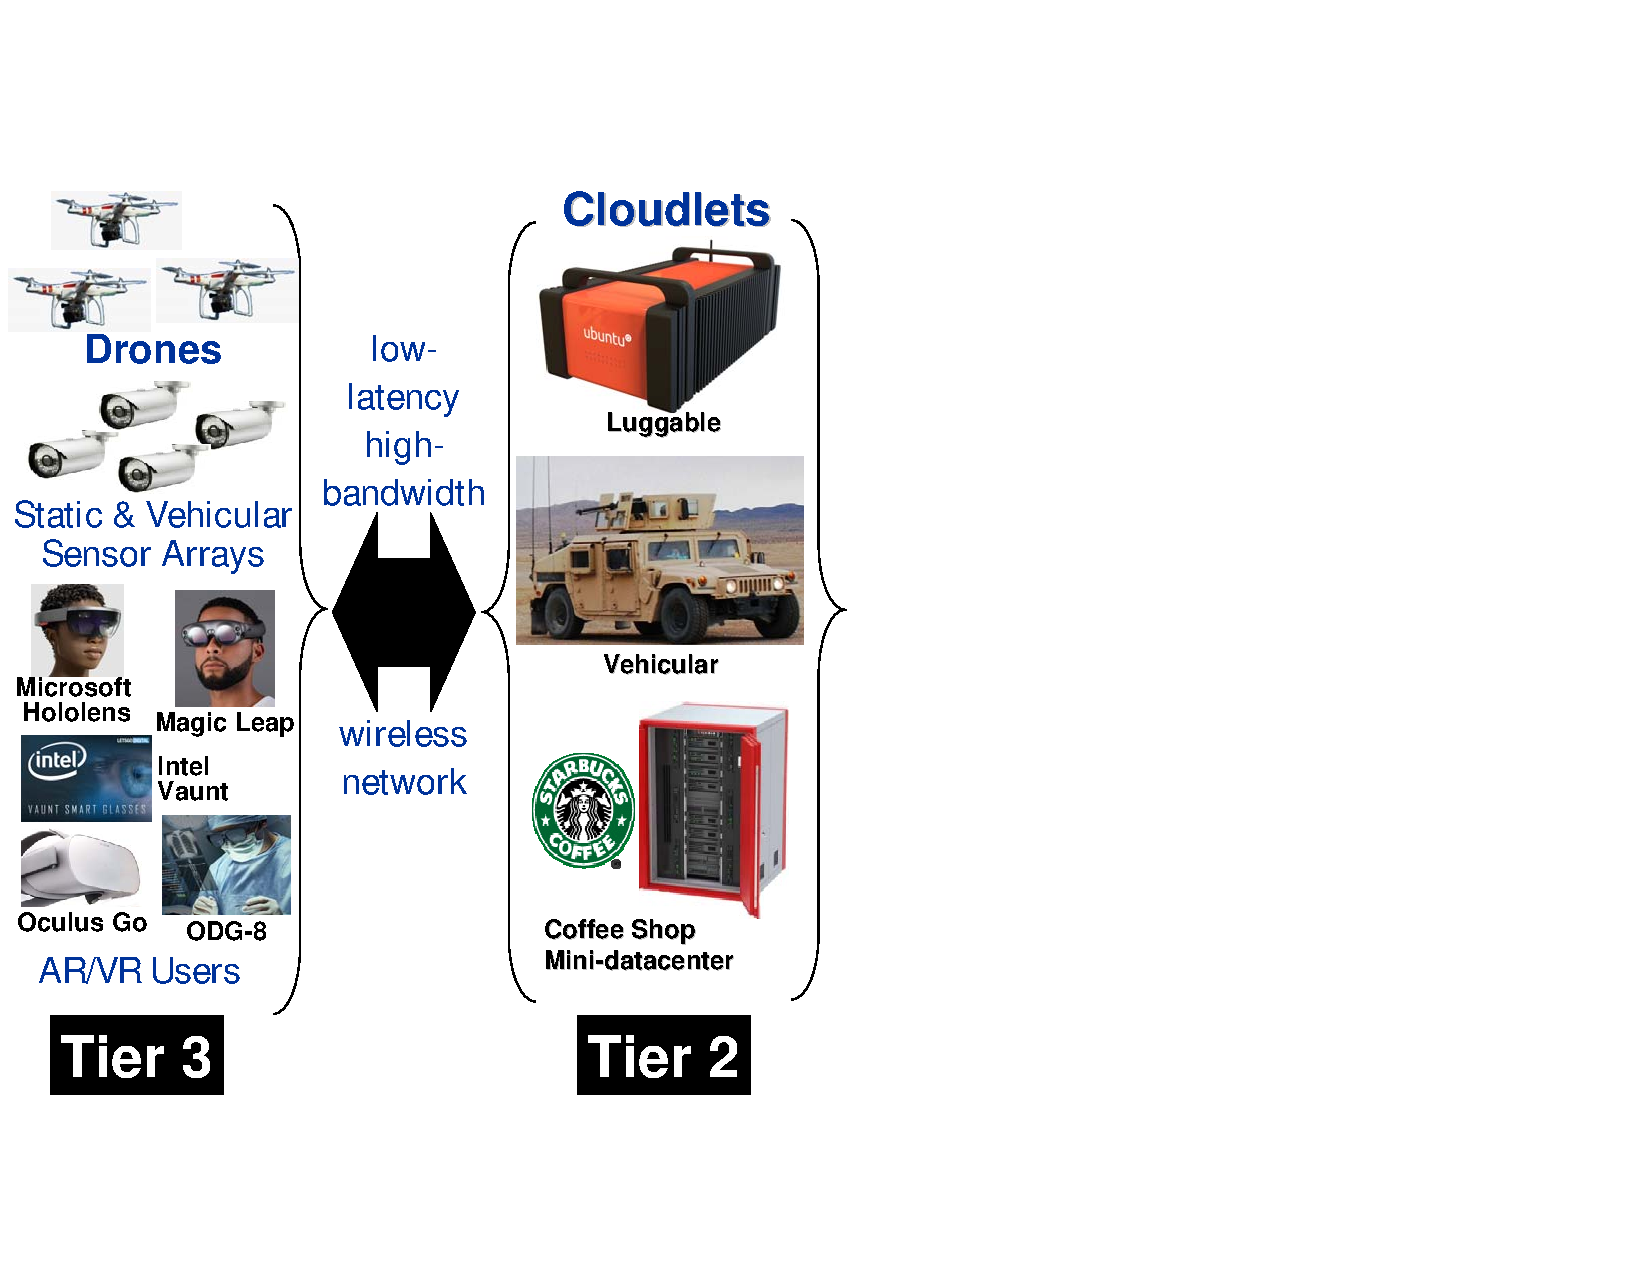
\includegraphics[scale=0.45]{FIGS/fig-3tier-A.pdf}
\end{minipage}
\begin{minipage}[c]{2.7in}
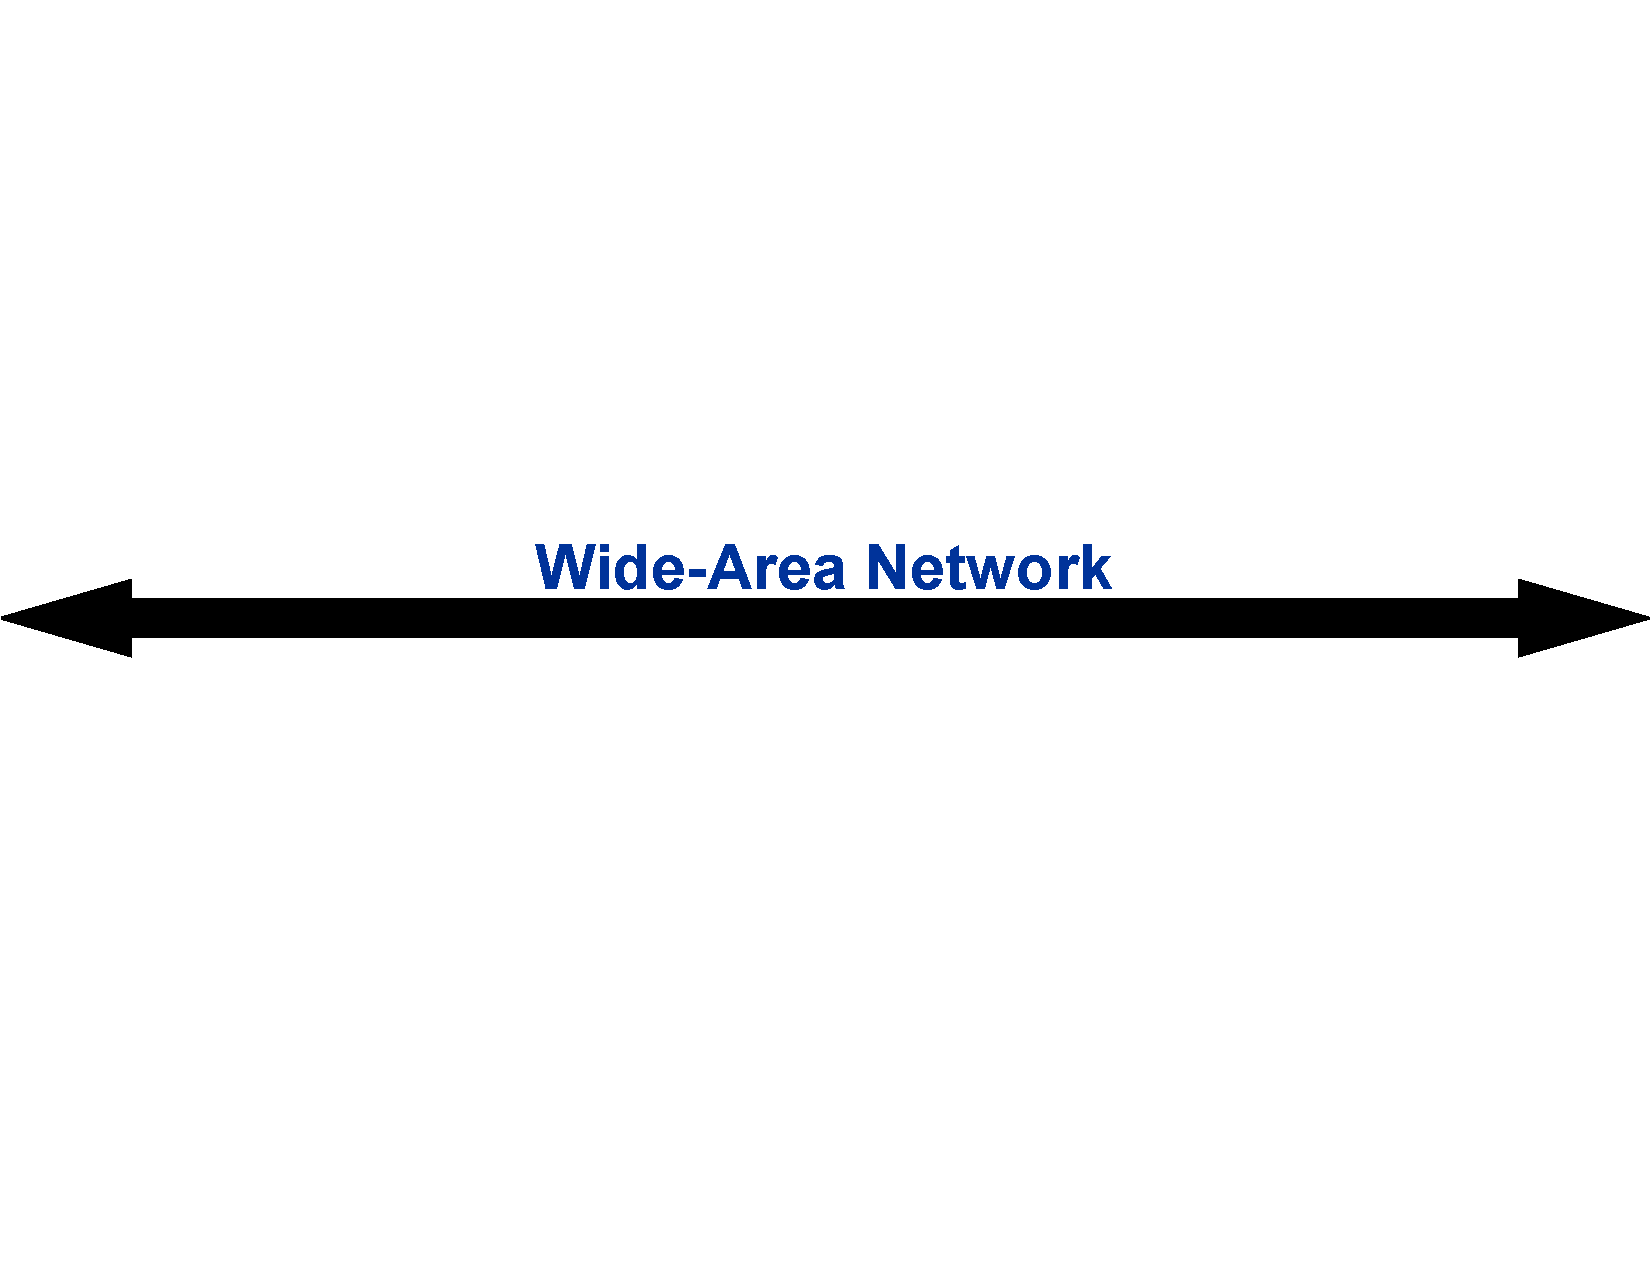
\includegraphics[scale=0.25]{FIGS/fig-3tier-B-cropped.pdf}\\
\end{minipage}
\begin{minipage}[c]{1in}
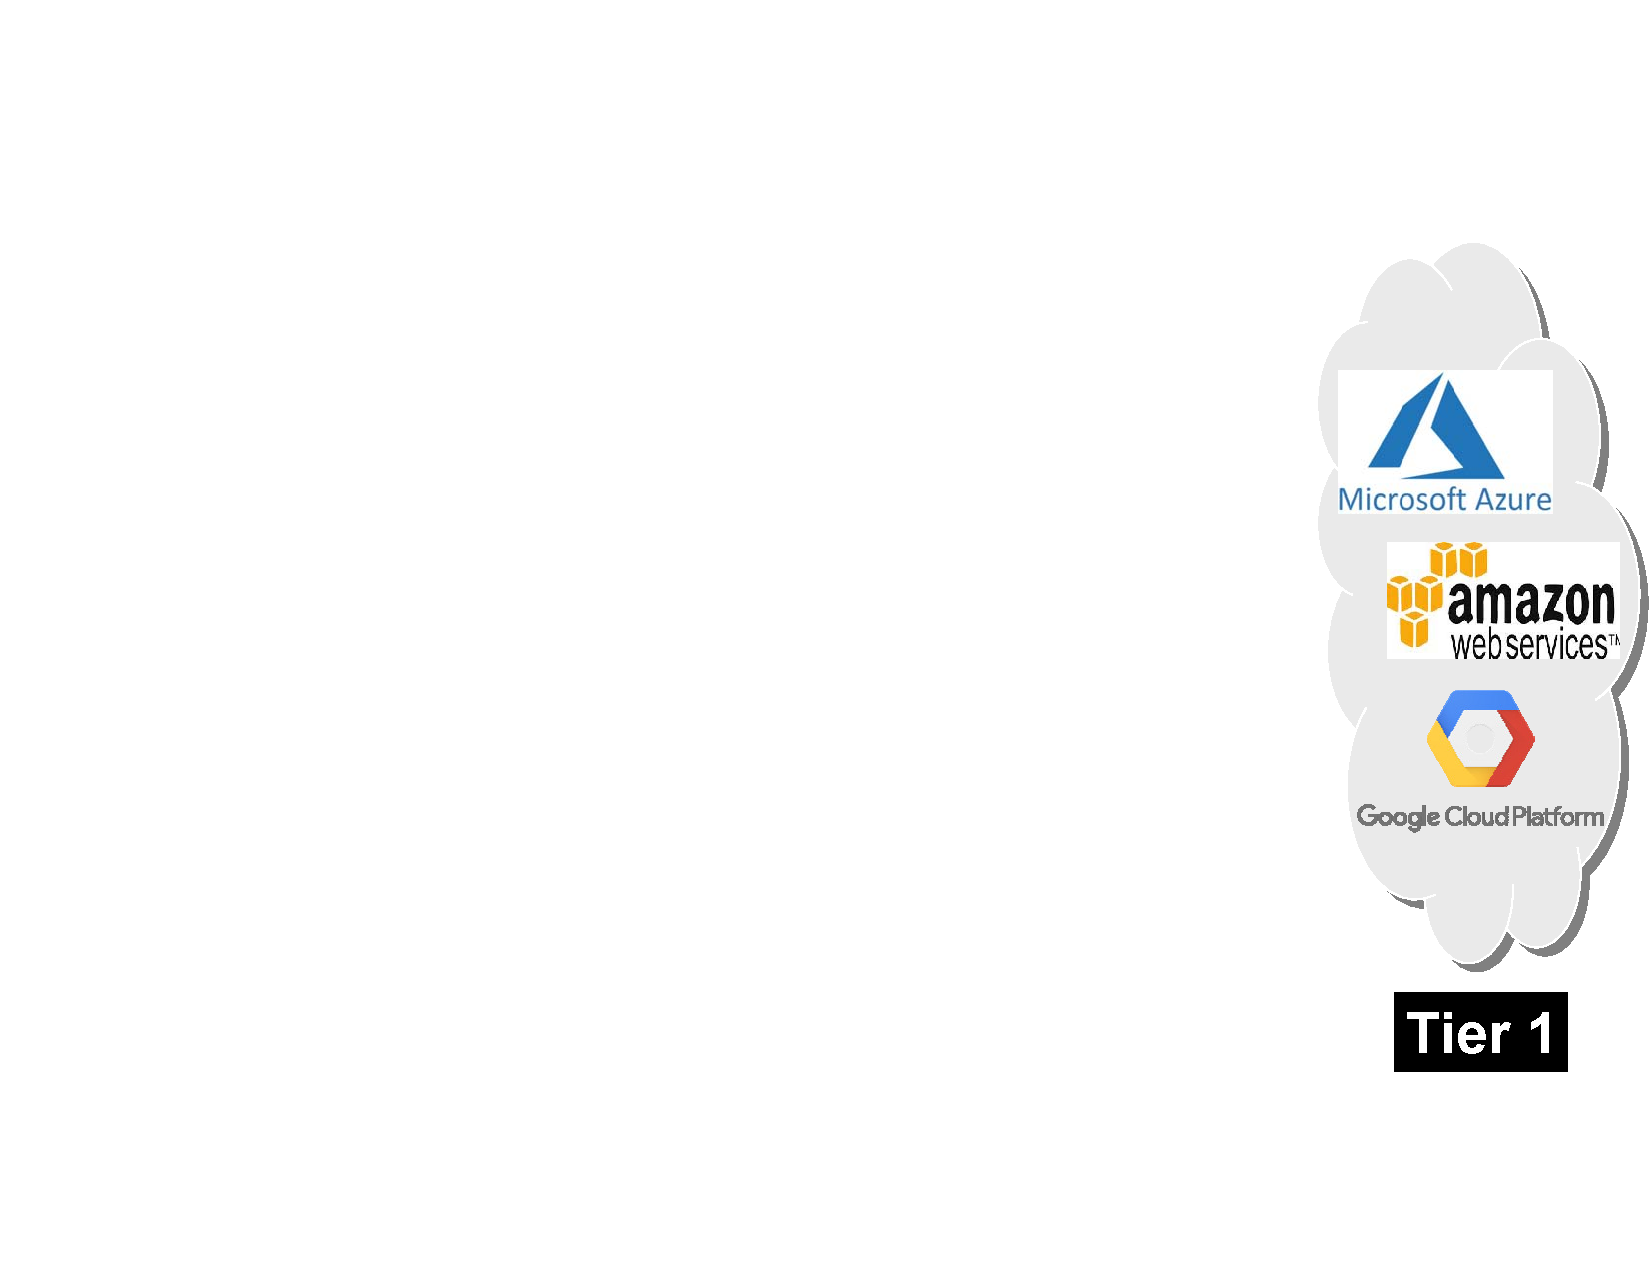
\includegraphics[scale=0.45]{FIGS/fig-3tier-C.pdf}
\end{minipage}
\centering
\captiontext{(Source: Satya et al~\cite{satya2019computing})}
\caption{Tiered Model of Computing}
\label{fig:3tier}
\end{figure*}

{\em Edge computing} is a nascent computing paradigm that has gained
considerable traction over the past few years. It champions the idea of placing
substantial compute and storage resources at the edge of the Internet, in close
proximity to mobile devices or sensors.  Terms such as
``cloudlets''~\cite{Satya2009}, ``micro data centers (MDCs)''~\cite{Greene2012},
``fog''~\cite{Bonomi2012}, and ``mobile edge computing (MEC)''~\cite{Brown2013}
are used to refer to these small, edge-located computing nodes.  We use these
terms interchangably in the rest of this dissertation. Edge computing is motivated by
its potential to improve latency, bandwidth, and scalability over a cloud-only
model.  More practically, some efforts stem from the drive towards
software-defined networking (SDN) and network function virtualization (NFV), and
the fact that the same hardware can provide SDN, NFV, and edge computing
services. This suggests that infrastructure providing edge computing services
may soon become ubiquitous, and may be deployed at greater densities than
content delivery network (CDN) nodes today. 

Satya et al.~\cite{satya2019computing} best describes the modern computing
landscape with edge computing using a tiered model, shown in
Figure~\ref{fig:3tier}. Tiers are separated by distinct yet stable sets of
design constraints. From left to right, this tiered model represents a hierarchy
of increasing physical size, compute power, energy usage, and elasticity. Tier-1
represents today's large-scale and heavily consolidated data-centers. Compute
elasticity and storage permanence are two dominating themes here. Tier-3
represents IoT and mobile devices, which are constrained by their physical size,
weight, and heat dissipation. Sensing is the key functionality of Tier-3
devices. For example, today's smartphones are already rich in sensors, including
camera, microphone, accelerometers, gyroscopes and GPS. In addition, an
increasing amount of IoT devices with specific sensing modalities are getting
adopted, e.g. smart speakers, security cameras, and smart thermostats. 

With the large-scale deployment of Tier-3 devices, there exists a tension
between the gigantic amount of data collected and generated by them and their
limited capabilities to process these data on-board. For example, most
surveillance cameras are limited in computation to run state-of-art computer
vision algorithms to analyze the videos they capture. To overcome this tension,
a Tier-3 device could offload computation over network to Tier-1. This
capability was first demonstrated in 1997 by Noble et al.~\cite{Noble1997}, who
used it to implement speech recognition with acceptable performance on a
resource-limited mobile device. In 1999, Flinn et al.~\cite{Flinn1999} extended
this approach to improve battery life.  These concepts were generalized in a
2001 paper that introduced the term {\em cyber foraging} for the amplification
of a mobile device's data or compute capabilities by leveraging nearby
infrastructure~\cite{Satya2001}.  Thanks to these research efforts, computation
offloading is widely used by IoT devices today. For example, when a user asks an
Amazon Echo smart speaker ``Alexa, what is the weather today?'', the user's
audio stream is captured by the smart speaker and transmitted to the cloud for
speech recognition, text understanding, and question answering.

However, offloading computation to the cloud has its own downside. Because of
the consolidation needed to achieve the economy of scale, today's datacenters
are ``far'' from Tier-3 devices. The latency, throughput, and cost of wide-area
network (WAN) significantly limit the amount of applications that can benefit
from computation offloading. Even worse, it is the logical distance in the
network that matters rather than the physical distance. Routing decisions in
today's Internet are made locally and are based on business agreements,
resulting in suboptimal solutions. For example, using traceroute, we determine
that a LTE packet originating from a smartphone on the campus of Carnegie Mellon
University (CMU) in Pittsburgh to a nearby server actually traverses to
Philedelphia, a city several hundreds miles away. This is because Philidephia
has the nearest peering point of the particular commercial LTE network in use to
the public Internet. In 2010, Li et al.~\cite{li2010cloudcmp} report that the
average round trip time (RTT) from 260 global vantage points to their optimal
Amazon EC2 instances is 74 ms. In addition to long network delay, the high
network fan-in of datacenters means its aggregation network needs to carry
significant amount of traffic. As the number of Tier-3 devices is expected to
grow exponentially, these network links face significant challenges to handle
the ever-increasing volume of ingress traffic. 

\begin{figure}
\begin{minipage}[c]{3in}
\begin{center}
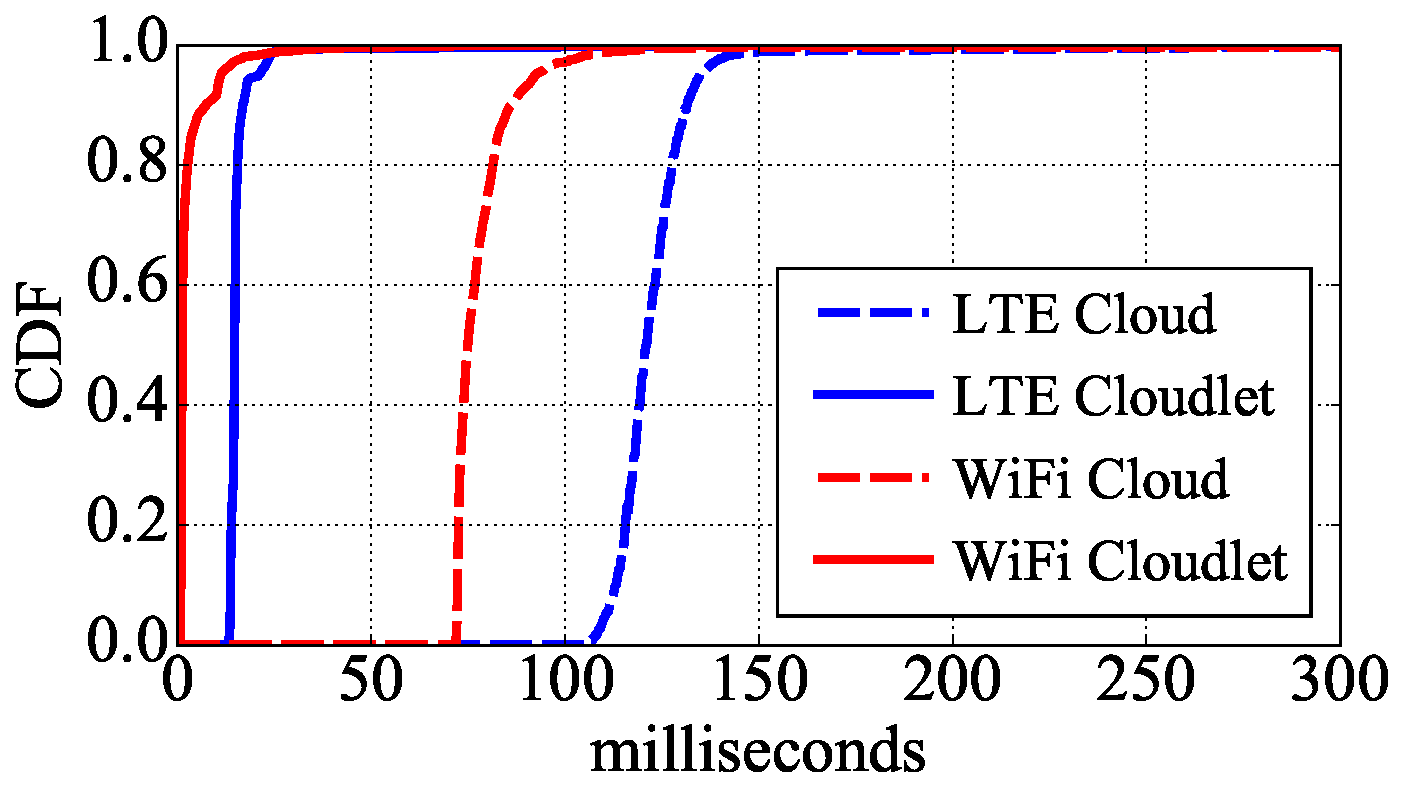
\includegraphics[height=1.5in]{FIGS/ping_cdf.pdf}
\captiontext{(Source: Hu et al~\cite{hu2016quantifying})}
\caption{CDF of pinging RTTs}
\label{fig:ping-CDF}
\end{center}
\end{minipage}
\begin{minipage}[c]{3.5in}
\begin{center}
    \hspace{0.2in}
    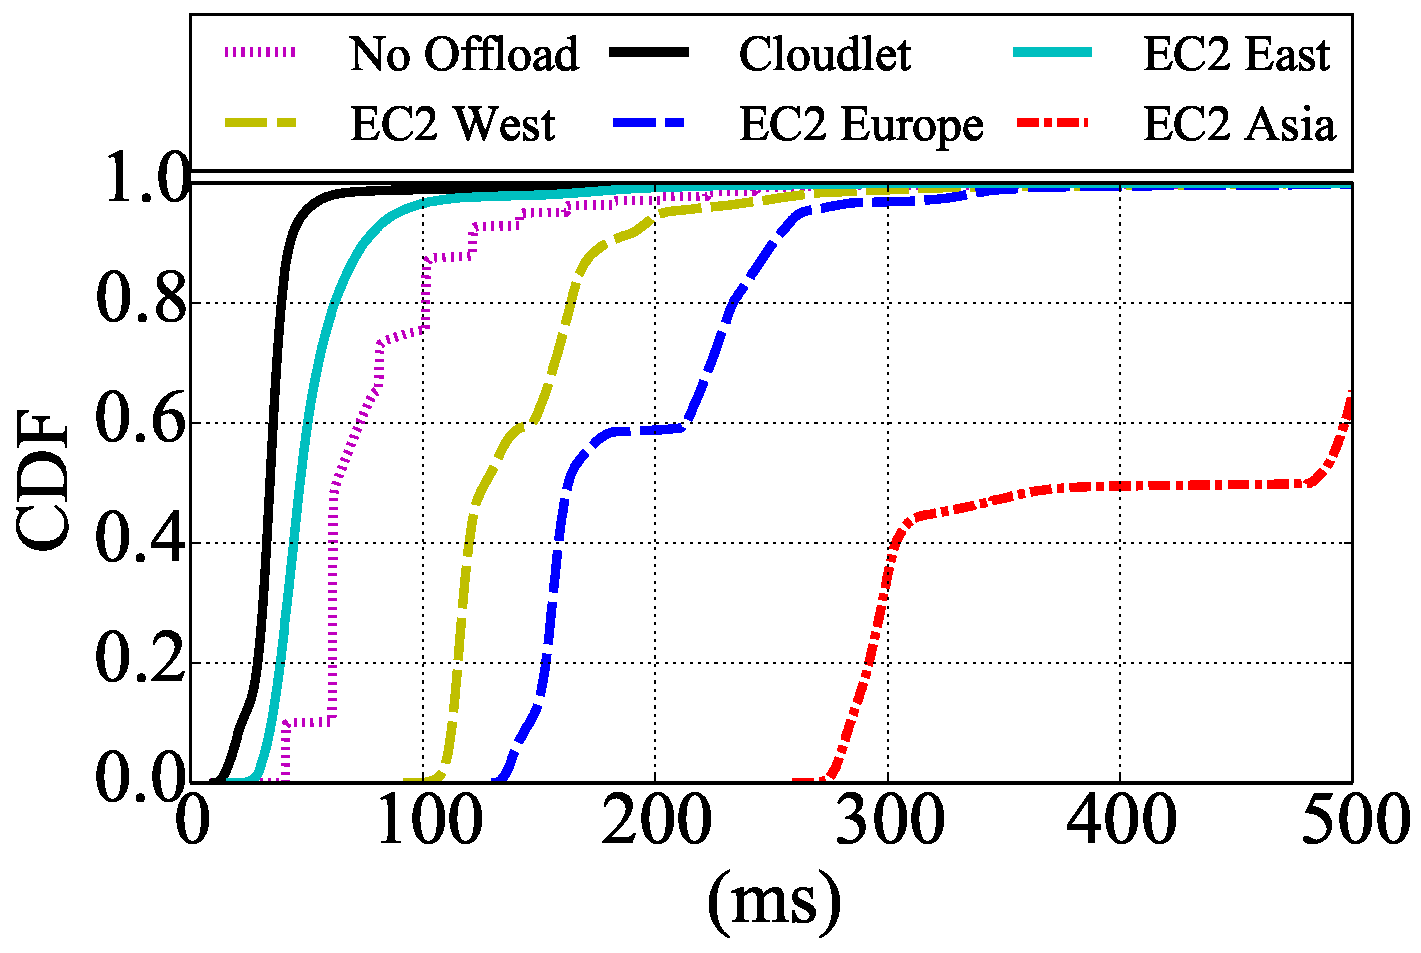
\includegraphics[width=0.8\textwidth,clip,trim=91pt 376pt 0 0]{FIGS/Legend-Wifi.pdf}
    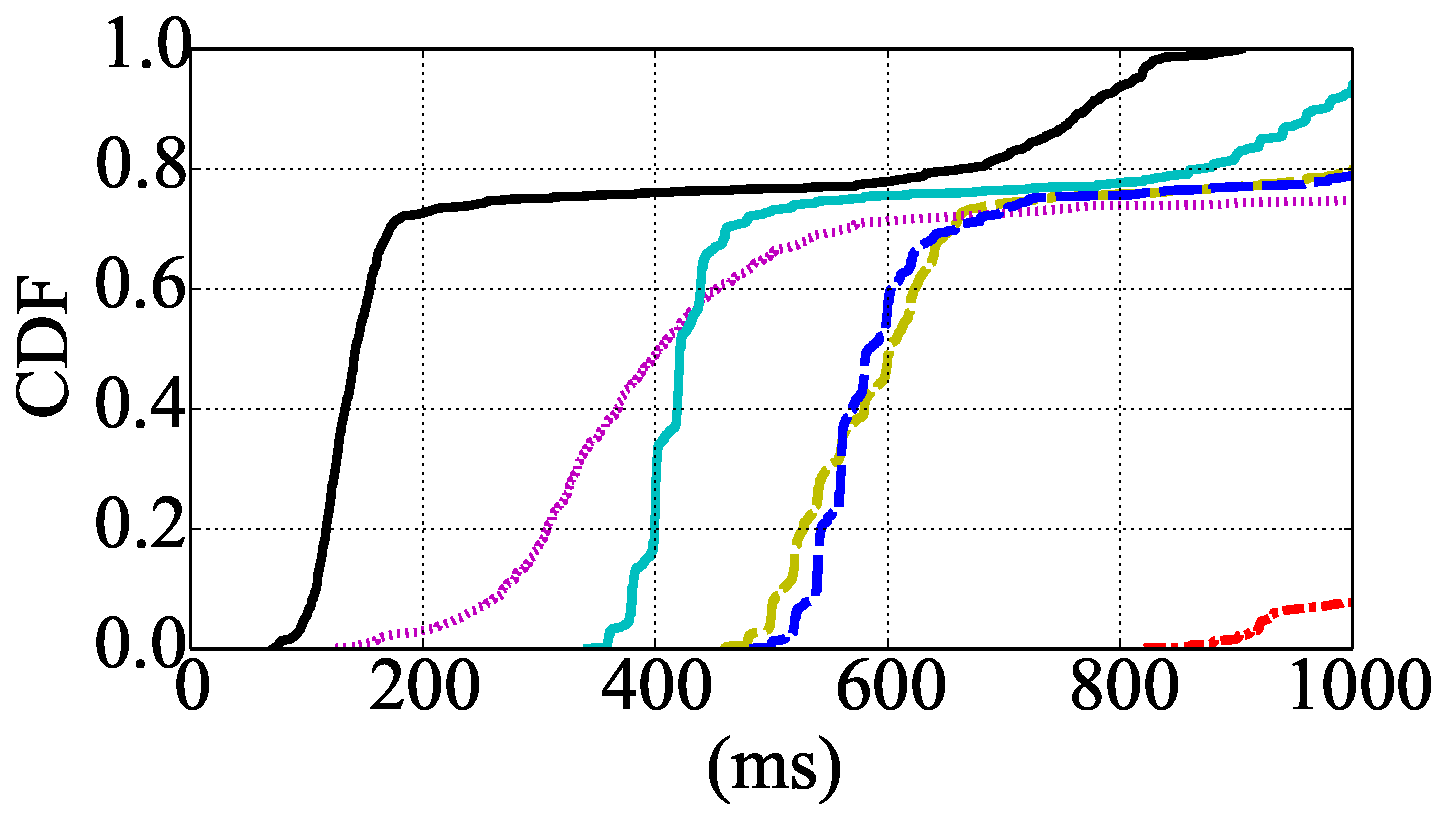
\includegraphics[width=3in]{FIGS/Face-LTE.pdf}
\captiontext{(Source: Hu et al~\cite{hu2016quantifying})}
\caption{FACE Response Time over LTE}
\label{fig:response-time-lte-face}
\end{center}
\end{minipage}
\end{figure}

To counter these problems, edge computing, shown as the Tier-2 in
Figure~\ref{fig:3tier}, is proposed. Cloudlets at Tier-2 creates the illusion of
bringing Tier-1 ``closer''. They are featured by their network proximity to
Tier-3 devices and their significantly larger compute and storage compared to
Tier-3 devices. While Tier-3 devices typically run on battery and are optimized
for low energy consumption, saving energy is not a major concern for Tier-2 as
they are either plugged into the electric grid or powered by other sources of
energy (e.g. fuels in a vehicle). Cloudlets serve two purposes in the tiered
model. First, they provide infrastructure for compute-intensive and
latency-sensitive applications for Tier-3. Wearable cognitive assistance is an
examplar of these applications. Second, by processing data closer to the source
of the content, it reduces the excessive traffic going into Tier-1 datacenters.
Figure~\ref{fig:ping-CDF} shows the RTT comparison of PING to the cloud and the
cloudlet over WiFi and LTE. Cloudlet's RTT is on average 80 to 100ms shorter
than its counterpart to the cloud. Figure~\ref{fig:response-time-lte-face} shows
the impact of network latency on an application that recognizes faces. Three
offloading scenarios are considered: offloading to the cloud, offloading to the
cloudlet, and no offloading. The data transmitted are images captured by a
smartphone. As we can see, the limited bandwidth of the cellular network further
worsen the response time when offloading to the cloud. In fact, for this
particular application, even local execution outperforms offloading to the
nearest cloud due to network delay. The optimal computational offload location
is cloudlet, whose median response time is more than 200ms faster than local
execution and about 250 ms faster than the nearest cloud.

The low-latency and high-bandwidth compute infrastructure provided by cloudlets
is an indispensible foundation for latency-sensitive and compute-intensive
wearable cognitive assistance. Cloudlet also poses unique challenges for
scalability as resources are a lot more limited compared to datacenters. How to
scale WCAs to many users using cloudlets is the key question we set out to
investigate in this dissertation. 


\section{Gabriel Platform}
\label{sec: bg-gabriel}

\begin{figure}
\centering
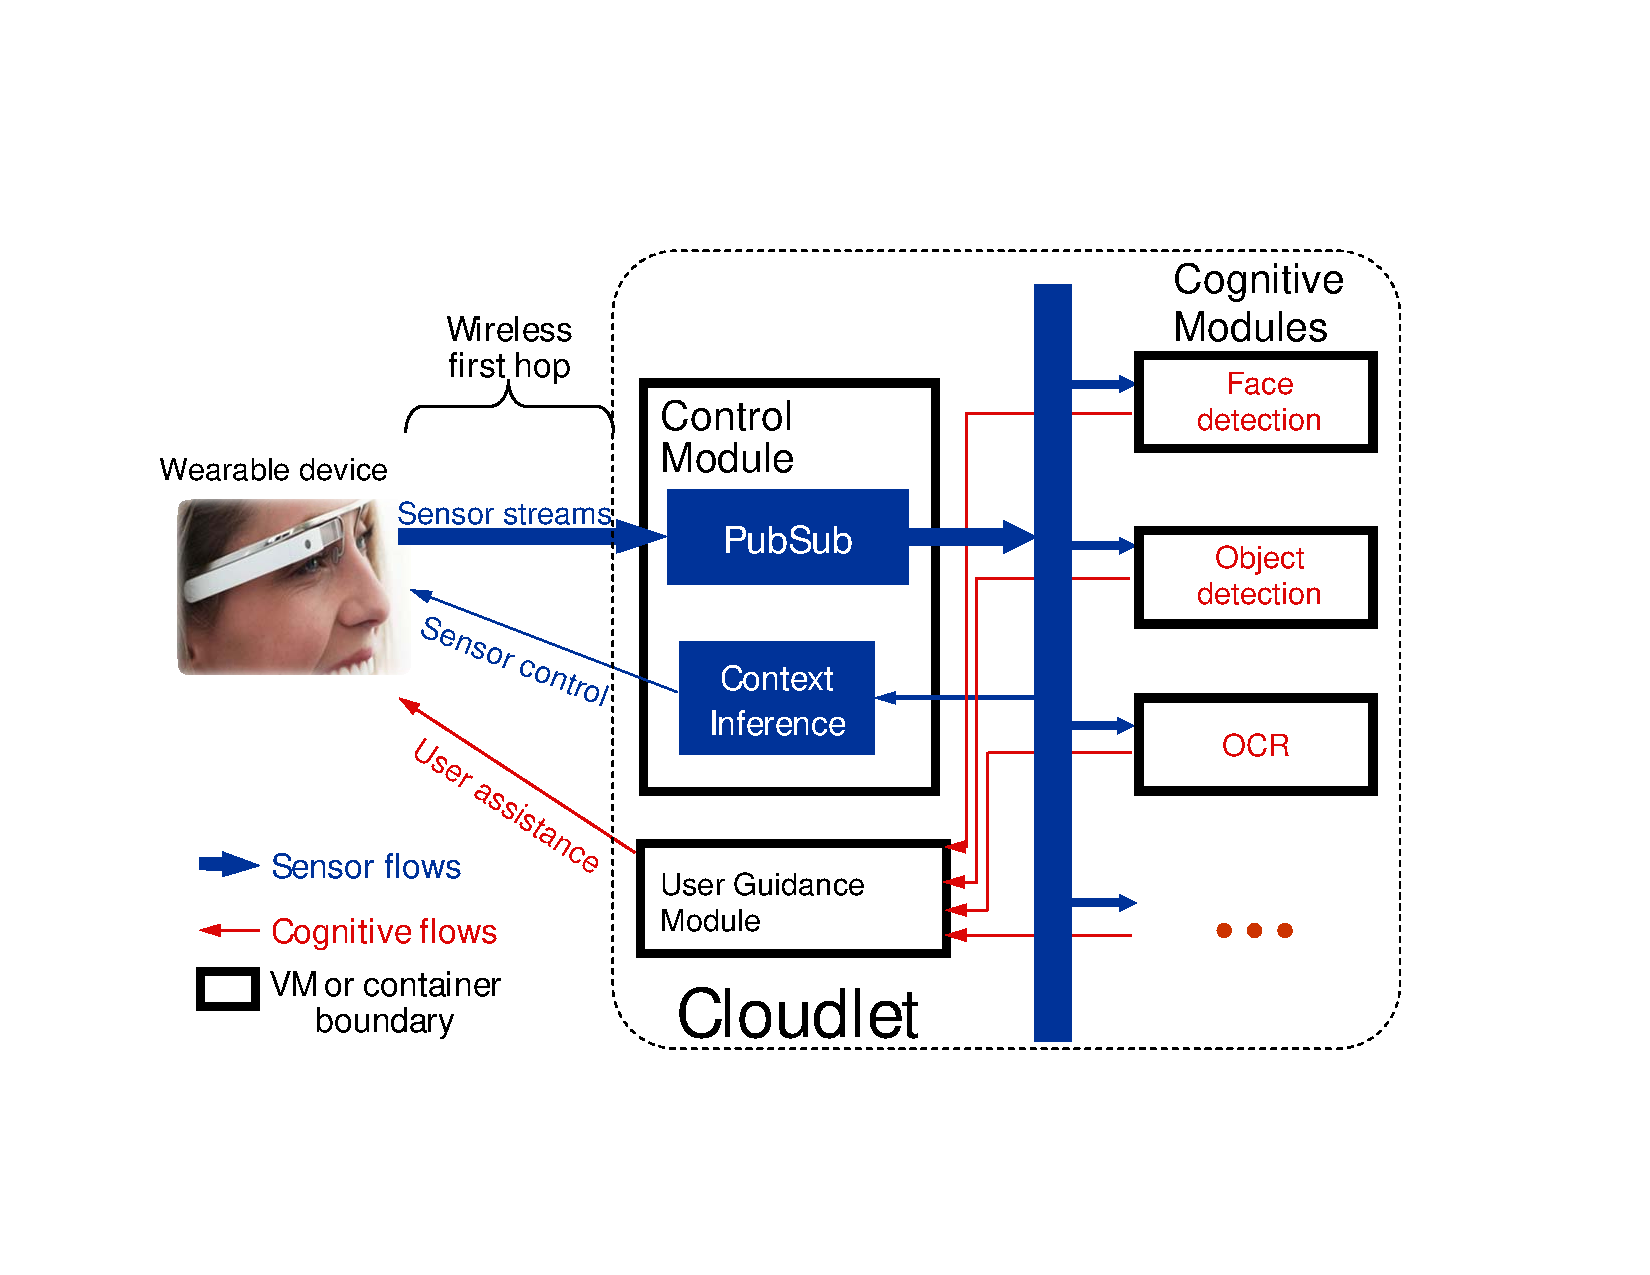
\includegraphics[width=0.8\linewidth]{FIGS/fig-backend-structure-simple-crop.pdf}
\begin{captiontext}
{\rm (Source: Chen et al~\cite{chen2017empirical})}
\end{captiontext}
\caption{Gabriel Platform}
\label{fig:gabriel}
\end{figure}

The Gabriel platform~\cite{ha2014towards,chen2017empirical}, shown in
Figure~\ref{fig:gabriel}, is the first application framework for wearable
cognitive assistance. It consists of a front-end running on wearable devices and
a back-end running on cloudlets. The Gabriel front-end performs preprocessing of
sensor data (e.g., compression and encoding), which it then streams over a
wireless network to a cloudlet.  The Gabriel back-end on the cloudlet has a
modular structure. The {\em control module} is the focal point for all
interactions with the wearable device and can be thought as an agent for a
particular client on the cloudlet. A publish-subscribe (PubSub) mechanism
distributes the incoming sensor streams to multiple {\em cognitive modules}
(e.g., task-specific computer vision algorithms) for concurrent processing.
Cognitive module outputs are integrated by a task-specific {\em user guidance
module} that performs higher-level cognitive processing such as inferring task
state, detecting errors, and generating guidance in one or more modalities
(e.g., audio, video, text, etc.). The Gabriel platform automatically discovers
cognitive engines on the local network via a universal plug-and-play (UPnP)
protocol. The platform is designed to run on a small cluster of machines with
each modules capable of being separated or co-located with other modules via
process, container, or virtual machine virtualization. 

The original Gabriel platform was built with a single user in mind, and did not
have mechanisms to share cloudlet resources in a controlled manner.  It did,
however, have a token-based transmission mechanism.  This limited a client to
only a small number of outstanding operations, thereby offering a simple form of
rate adaptation to processing or network bottlenecks.  We have retained this
token mechanism in our system, described in the rest of this dissertation. In
addition, we have extended Gabriel with new mechanisms to handle multi-tenancy,
perform resource allocation, and support application-aware adaptation.  We refer
to the two versions of the platform as ``Original Gabriel'' and ``Scalable
Gabriel.''

\section{Example Gabriel Applications}
\label{sec:example-apps}

Many applications have been built on top of the Gabriel platform.
Figure~\ref{fig:bg-apps-table} provides a summary of applications built by Chen
et al~\cite{chen2018application}. These applications run on multiple wearable
devices such as Google Glass, Microsoft HoloLens, Vuzix Glass, and ODG R7. The
cloudlet processing of these applications consists of two major phases. The
first phase uses computer vision to extract a symbolic, idealized representation
of the state of the task, accounting for real-world variations in lighting,
viewpoint, etc.  The second phase operates on the symbolic representation,
implements the logic of the task at hand, and occasionally generates guidance
for the user.  In most WCA applications, the first phase is far more compute
intensive than the second phase. While visual data is the focus of the analysis,
other types of sensor data, e.g. audio, are also used to help infer user states.

Building on lessons learned by Chen et al~\cite{chen2018application}, we create
and implement several real-life WCA applications whose tasks are more complex.
They also pose more challenges to the computer vision processing as the parts
are not designed for machine recognition. In particular, we focus on assembly
tasks. Many assembly tasks, including manufacturing assembly and medical
procedures, are tedious and error-prone. WCAs can help reduce errors, provide
training, and assist human operators by continuously monitoring their actions
and offering feedback. We describe two of these applications below in detail.

\begin{figure*}
\begin{tabular}{|p{0.31in}|p{0.95in}|p{3.5in}|p{0.84in}|p{0.8in}|}
\hline
App Name & Example Input Video Frame & Description & Symbolic \phantom{000} Representation & Example Guidance \\
\hline
\phantom{000} \textbf{Pool}     & \raisebox{-0.9\totalheight}{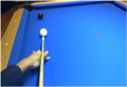
\psfig{file=FIGS/bigtable2/example-pool.png, width=0.97in}}
&
Helps a novice pool player aim correctly. Gives continuous visual feedback (left arrow, right arrow, or thumbs up) as the user turns his cue stick. Correct shot angle is calculated based on fractional aiming system~\cite{FractionalAiming}. Color, line, contour, and shape detection are used. The symbolic representation describes the positions of the balls, target pocket, and the top and bottom of cue stick.
&
\phantom{000} $<$Pocket, object ball, cue ball, cue top, cue bottom$>$ & \phantom{000} \raisebox{-0.85\totalheight}{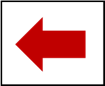
\psfig{file=FIGS/bigtable2/guidance-pool.png, width=0.8in}} \\
\hline
\phantom{000} \textbf{Ping-pong} & \raisebox{-0.9\totalheight}{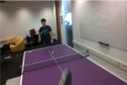
\psfig{file=FIGS/bigtable2/example-pingpong.png, width=0.97in}}
&
Tells novice to hit ball to the left or right, depending on which is more likely to beat opponent. Uses color, line and optical-flow based motion detection to detect ball, table, and opponent. The symbolic representation is a 3-tuple: in rally or not, opponent position, ball position. Whispers ``left'' or ``right'' or offers spatial audio guidance using~\cite{tang2014assistive}.

    Video URL: {\em \href{https://youtu.be/\_lp32sowyUA}{https://youtu.be/\_lp32sowyUA}}
&
\phantom{000} $<$InRally, ball position, opponent position$>$ & \phantom{000} Whispers ``Left!'' \\
\hline
\phantom{000} \textbf{Work-out} & \raisebox{-0.9\totalheight}{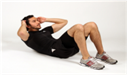
\psfig{file=FIGS/bigtable2/example-workout.png, width=0.97in}}
&
Guides correct user form in exercise actions like sit-ups and push-ups, and counts out repetitions. Uses Volumetric Template Matching~\cite{ke2007event} on a 10-15 frame video segment to classify the exercise.
%A poorly-performed repetition is classified as a distinct type of exercise (e.g. ``good pushup'' versus ``bad pushup'').
Uses smart phone on the floor for third-person viewpoint.
&
\phantom{000} $<$Action, count$>$ & \phantom{000} Says ``8 '' \\
\hline
\phantom{000} \textbf{Face}     & \raisebox{-0.9\totalheight}{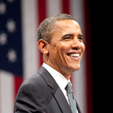
\psfig{file=FIGS/bigtable2/example-face.png, width=0.97in}}
&
Jogs your memory on a familiar face whose name you cannot recall. Detects and extracts a tightly-cropped image of each face, and then applies a state-of-art face recognizer using deep residual network~\cite{he2016deep}. Whispers the name of a person.
Can be used in combination with Expression~\cite{anam2014expression} to offer conversational hints.
&
\phantom{000} ASCII text of name & \phantom{000} Whispers ``Barack Obama'' \\
\hline
\phantom{000} \textbf{Lego} & \raisebox{-0.9\totalheight}{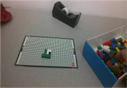
\psfig{file=FIGS/bigtable2/example-lego.png, width=0.97in}}
&
Guides a user in assembling 2D Lego models. Each video frame is analyzed in three steps: (i) finding the board using its distinctive color and black dot pattern; (ii) locating the Lego bricks on the board using edge and color detection; (iii) assigning brick color using weighted majority voting within each block. Color normalization is needed. The symbolic representation is a matrix representing color for each brick.

    Video URL: {\em \href{https://youtu.be/7L9U-n29abg}{https://youtu.be/7L9U-n29abg}}
&
\phantom{000} [[0, 2, 1, 1], \break [0, 2, 1, 6], \break [2, 2, 2, 2]] \break & \raisebox{-0.85\totalheight}{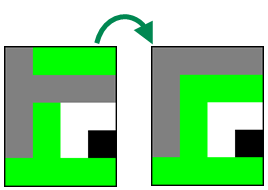
\psfig{file=FIGS/bigtable2/guidance-lego.png, width=0.8in}} Says ``Put a 1x3 green piece on top'' \\
\hline
\phantom{000} \textbf{Draw} & \raisebox{-0.9\totalheight}{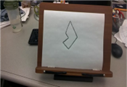
\psfig{file=FIGS/bigtable2/example-draw.png, width=0.97in}}
&
Helps a user to sketch better. Builds on third-party app~\cite{Iarussi2013} that was originally designed to take input sketches from pen-tablets and to output feedback on a desktop screen. Our implementation preserves the back-end logic. A new Glass-based front-end allows a user to use any drawing surface and instrument. Displays the error alignment in sketch on Glass.

    Video URL: {\em \href{https://youtu.be/nuQpPtVJC6o}{https://youtu.be/nuQpPtVJC6o}}
&
\raisebox{-0.85\totalheight}{
\psfig{file=FIGS/bigtable2/symbolic-draw.png, width=0.7in}} & \raisebox{-0.85\totalheight}{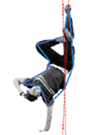
\psfig{file=FIGS/bigtable2/guidance-draw.png, width=0.8in}} \\
\hline
\phantom{000} \textbf{Sand-wich} & \raisebox{-0.9\totalheight}{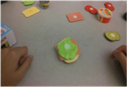
\psfig{file=FIGS/bigtable2/example-sandwich.png, width=0.97in}}
&
Helps a cooking novice prepare sandwiches according to a recipe. Since real food is perishable, we use a food toy with plastic ingredients. Object detection follows the state-of-art faster-RCNN deep neural net approach~\cite{ren2015faster}. Implementation is on top of Caffe~\cite{jia2014caffe} and Dlib~\cite{dlib09}. Transfer learning~\cite{Pan2010} helped us save time in labeling data and in training.

    Video URL: {\em \href{https://youtu.be/USakPP45WvM}{https://youtu.be/USakPP45WvM}}
&
\phantom{000} Object: \break ``E.g. Lettuce on top of ham and bread'' & \raisebox{-0.9\totalheight}{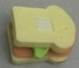
\psfig{file=FIGS/bigtable2/guidance-sandwich.jpg, width=0.7in}} Says ``Put a piece of bread on the lettuce'' \\
\hline

\end{tabular}
\caption{Prototype Wearable Cognitive Assistance Applications}
\label{fig:bg-apps-table}
\end{figure*}

\begin{figure}
\centering
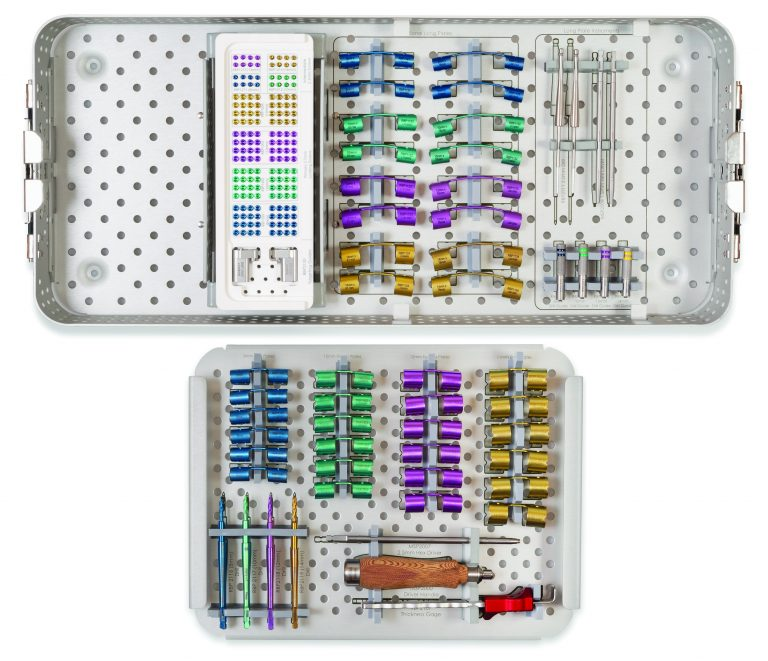
\includegraphics[width=0.5\linewidth]{FIGS/RibLoc.jpg}
\caption{RibLoc Kit}
\label{fig:ribloc}
\end{figure}

\begin{figure}
\centering
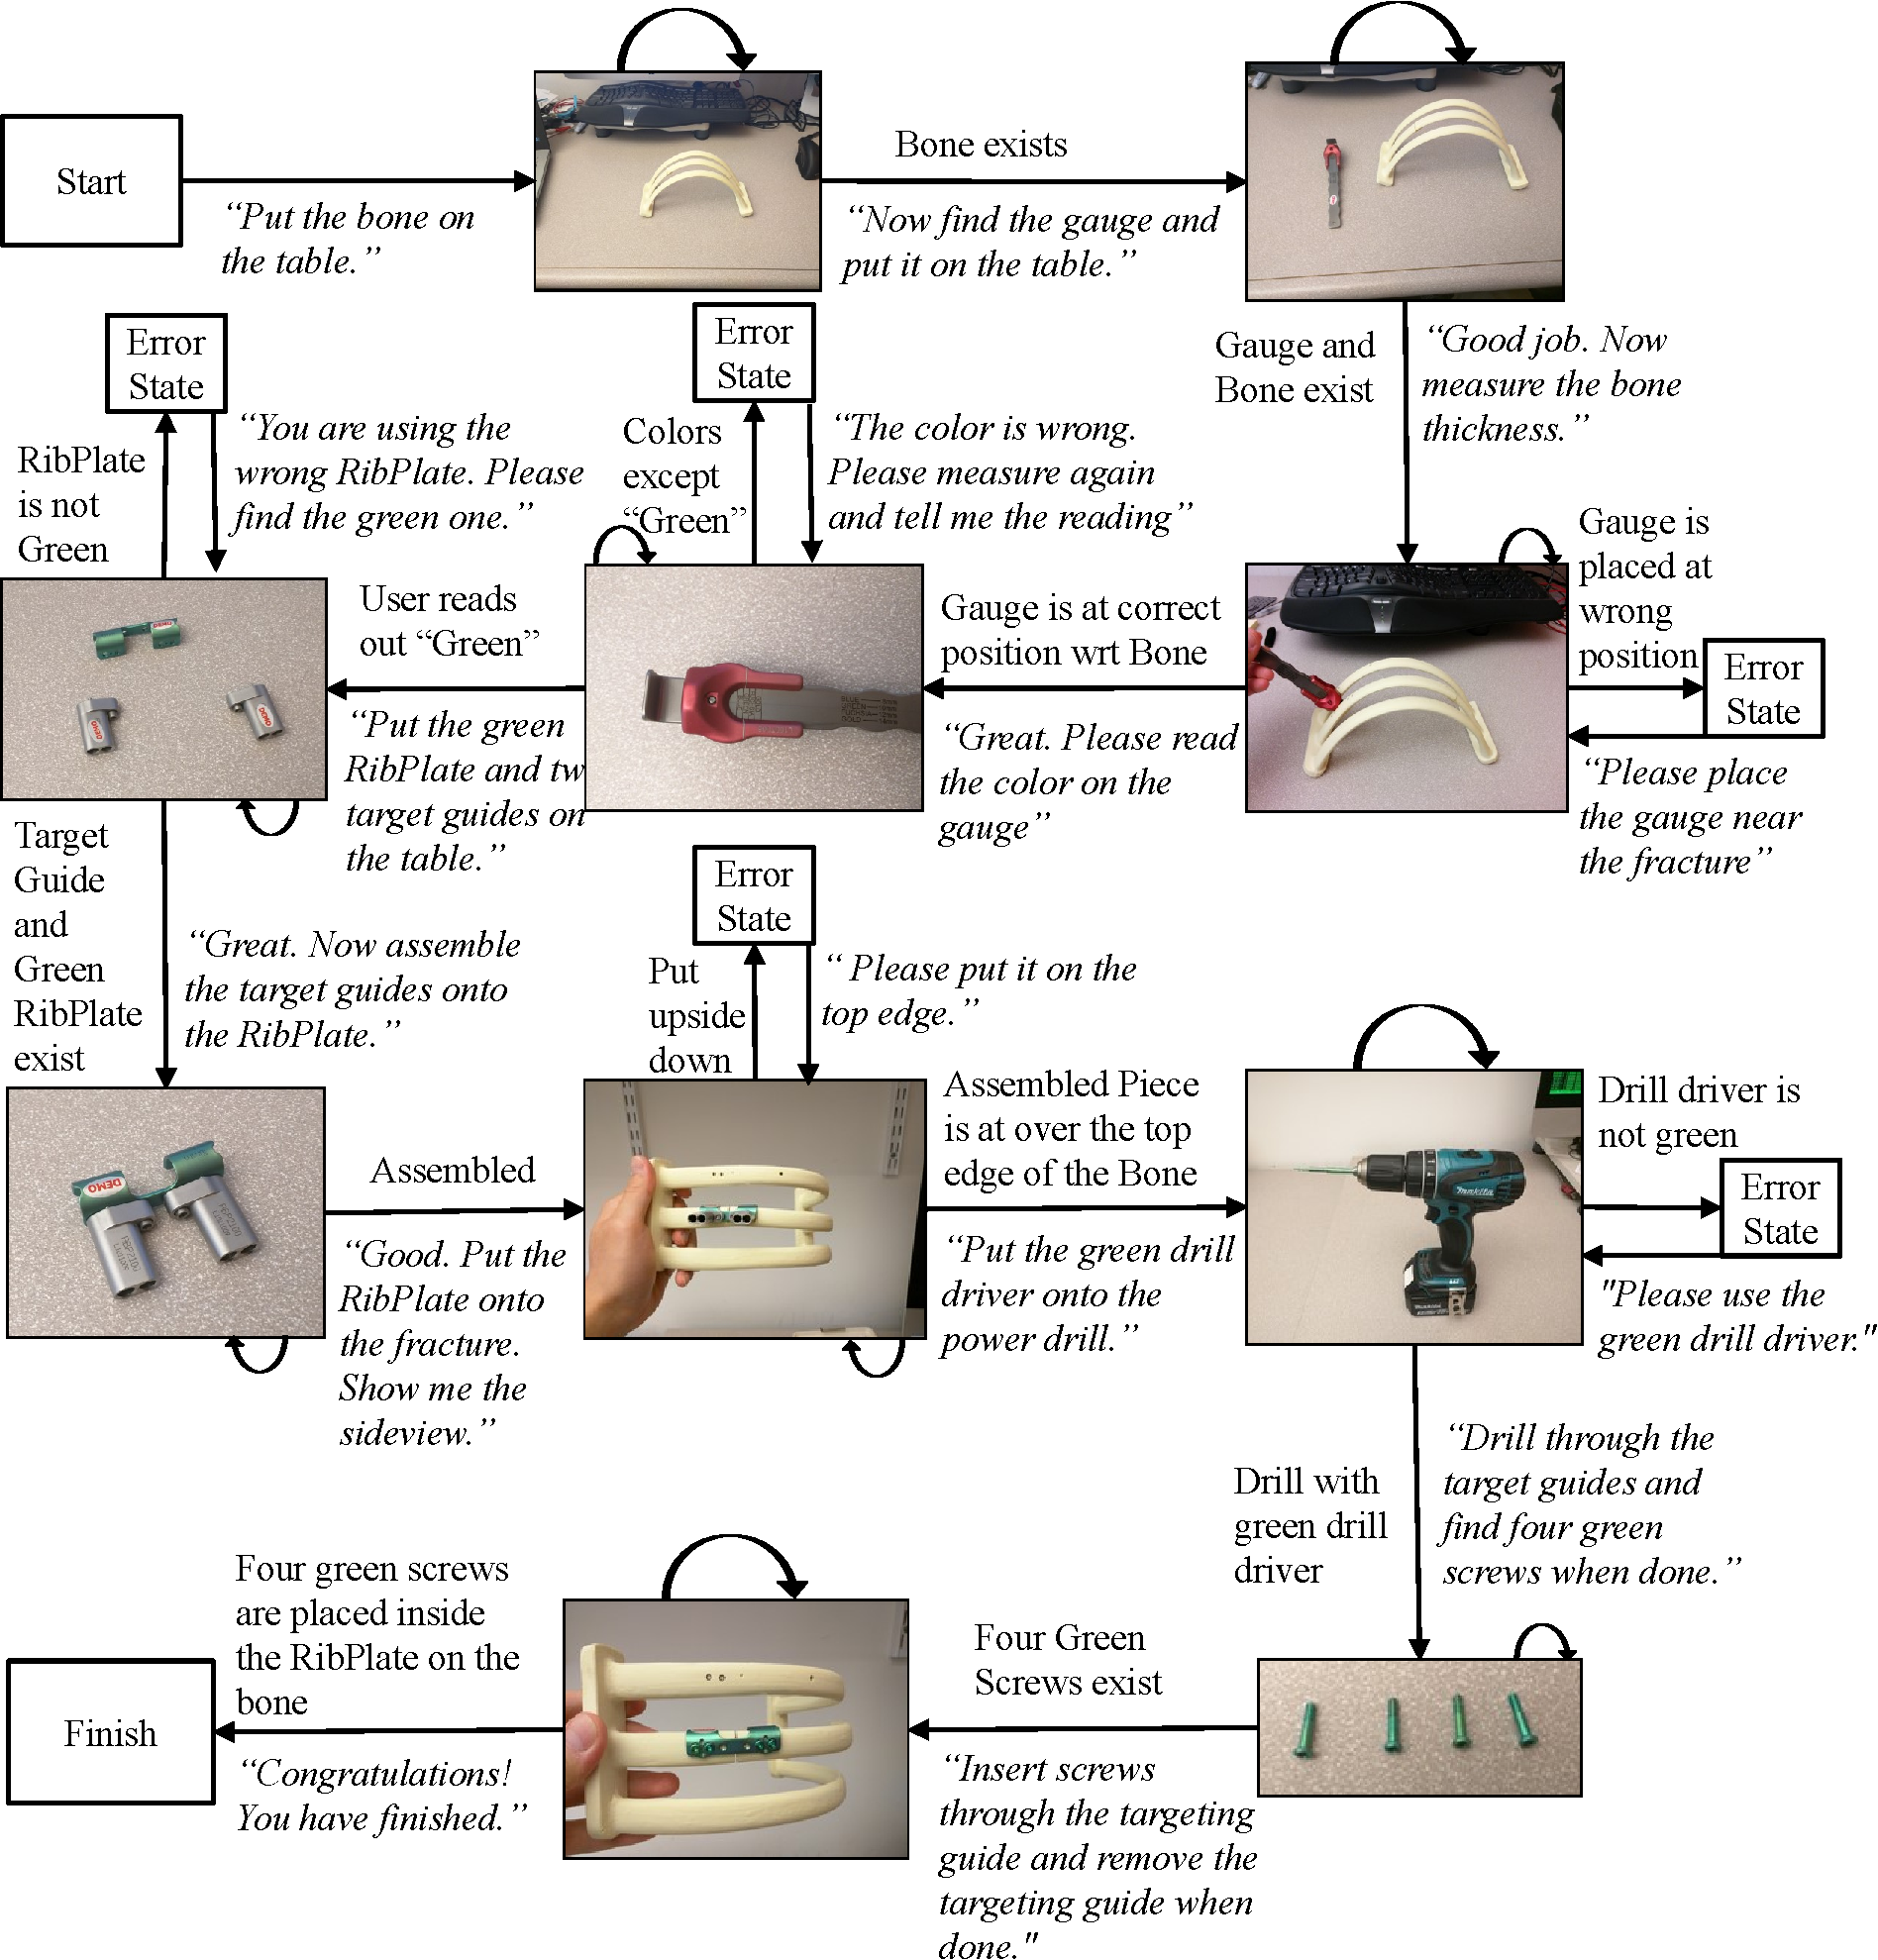
\includegraphics[width=\linewidth]{FIGS/ribloc-fsm-crop.pdf}
\caption{RibLoc Assistant Workflow}
\label{fig:ribloc-app}
\end{figure}

\subsection{RibLoc Application}

RibLoc Fracture Plating System~\cite{ribloc}, shown in Figure~\ref{fig:ribloc}
is used by surgeons to stabilize broken ribs for fracture repair. The surgery
consists of five major steps: measure ribs thickness, prepare the plate, drill
bone for screw insertion, insert screws, and tighten screws. To train doctors
how to use this kit, Acute Innovations, the manufacturer of RibLoc, currently
send sales personnel to doctors' office, often for extended period of time. To
reduce the cost of training, we develop a WCA for RibLoc that guides a surgeon
to learn RibLoc step-by-step on fake bones. Figure~\ref{fig:ribloc-app} shows
the task steps of the application as a finite state machine (FSM). Conditions of
state transitions are shown above the transition arrows and instructions given
to users are quoted in italics. Most of user state recognition is achieved by
verifying the existence and locations of key objects. One exception is rib
thickness measurement. The application asks the user to read out some text from
the gauge. Automatic speech recognition (ASR) is used to detect the user's
read-out. ASR is used because the text on the gauge has a low contrast with the
background that they are too hard to optical character recognition (OCR). A demo
video of RibLoc WCA is at \url{https://youtu.be/YRTXUty2P1U}.

\subsection{DiskTray Application}

\begin{figure}
\centering
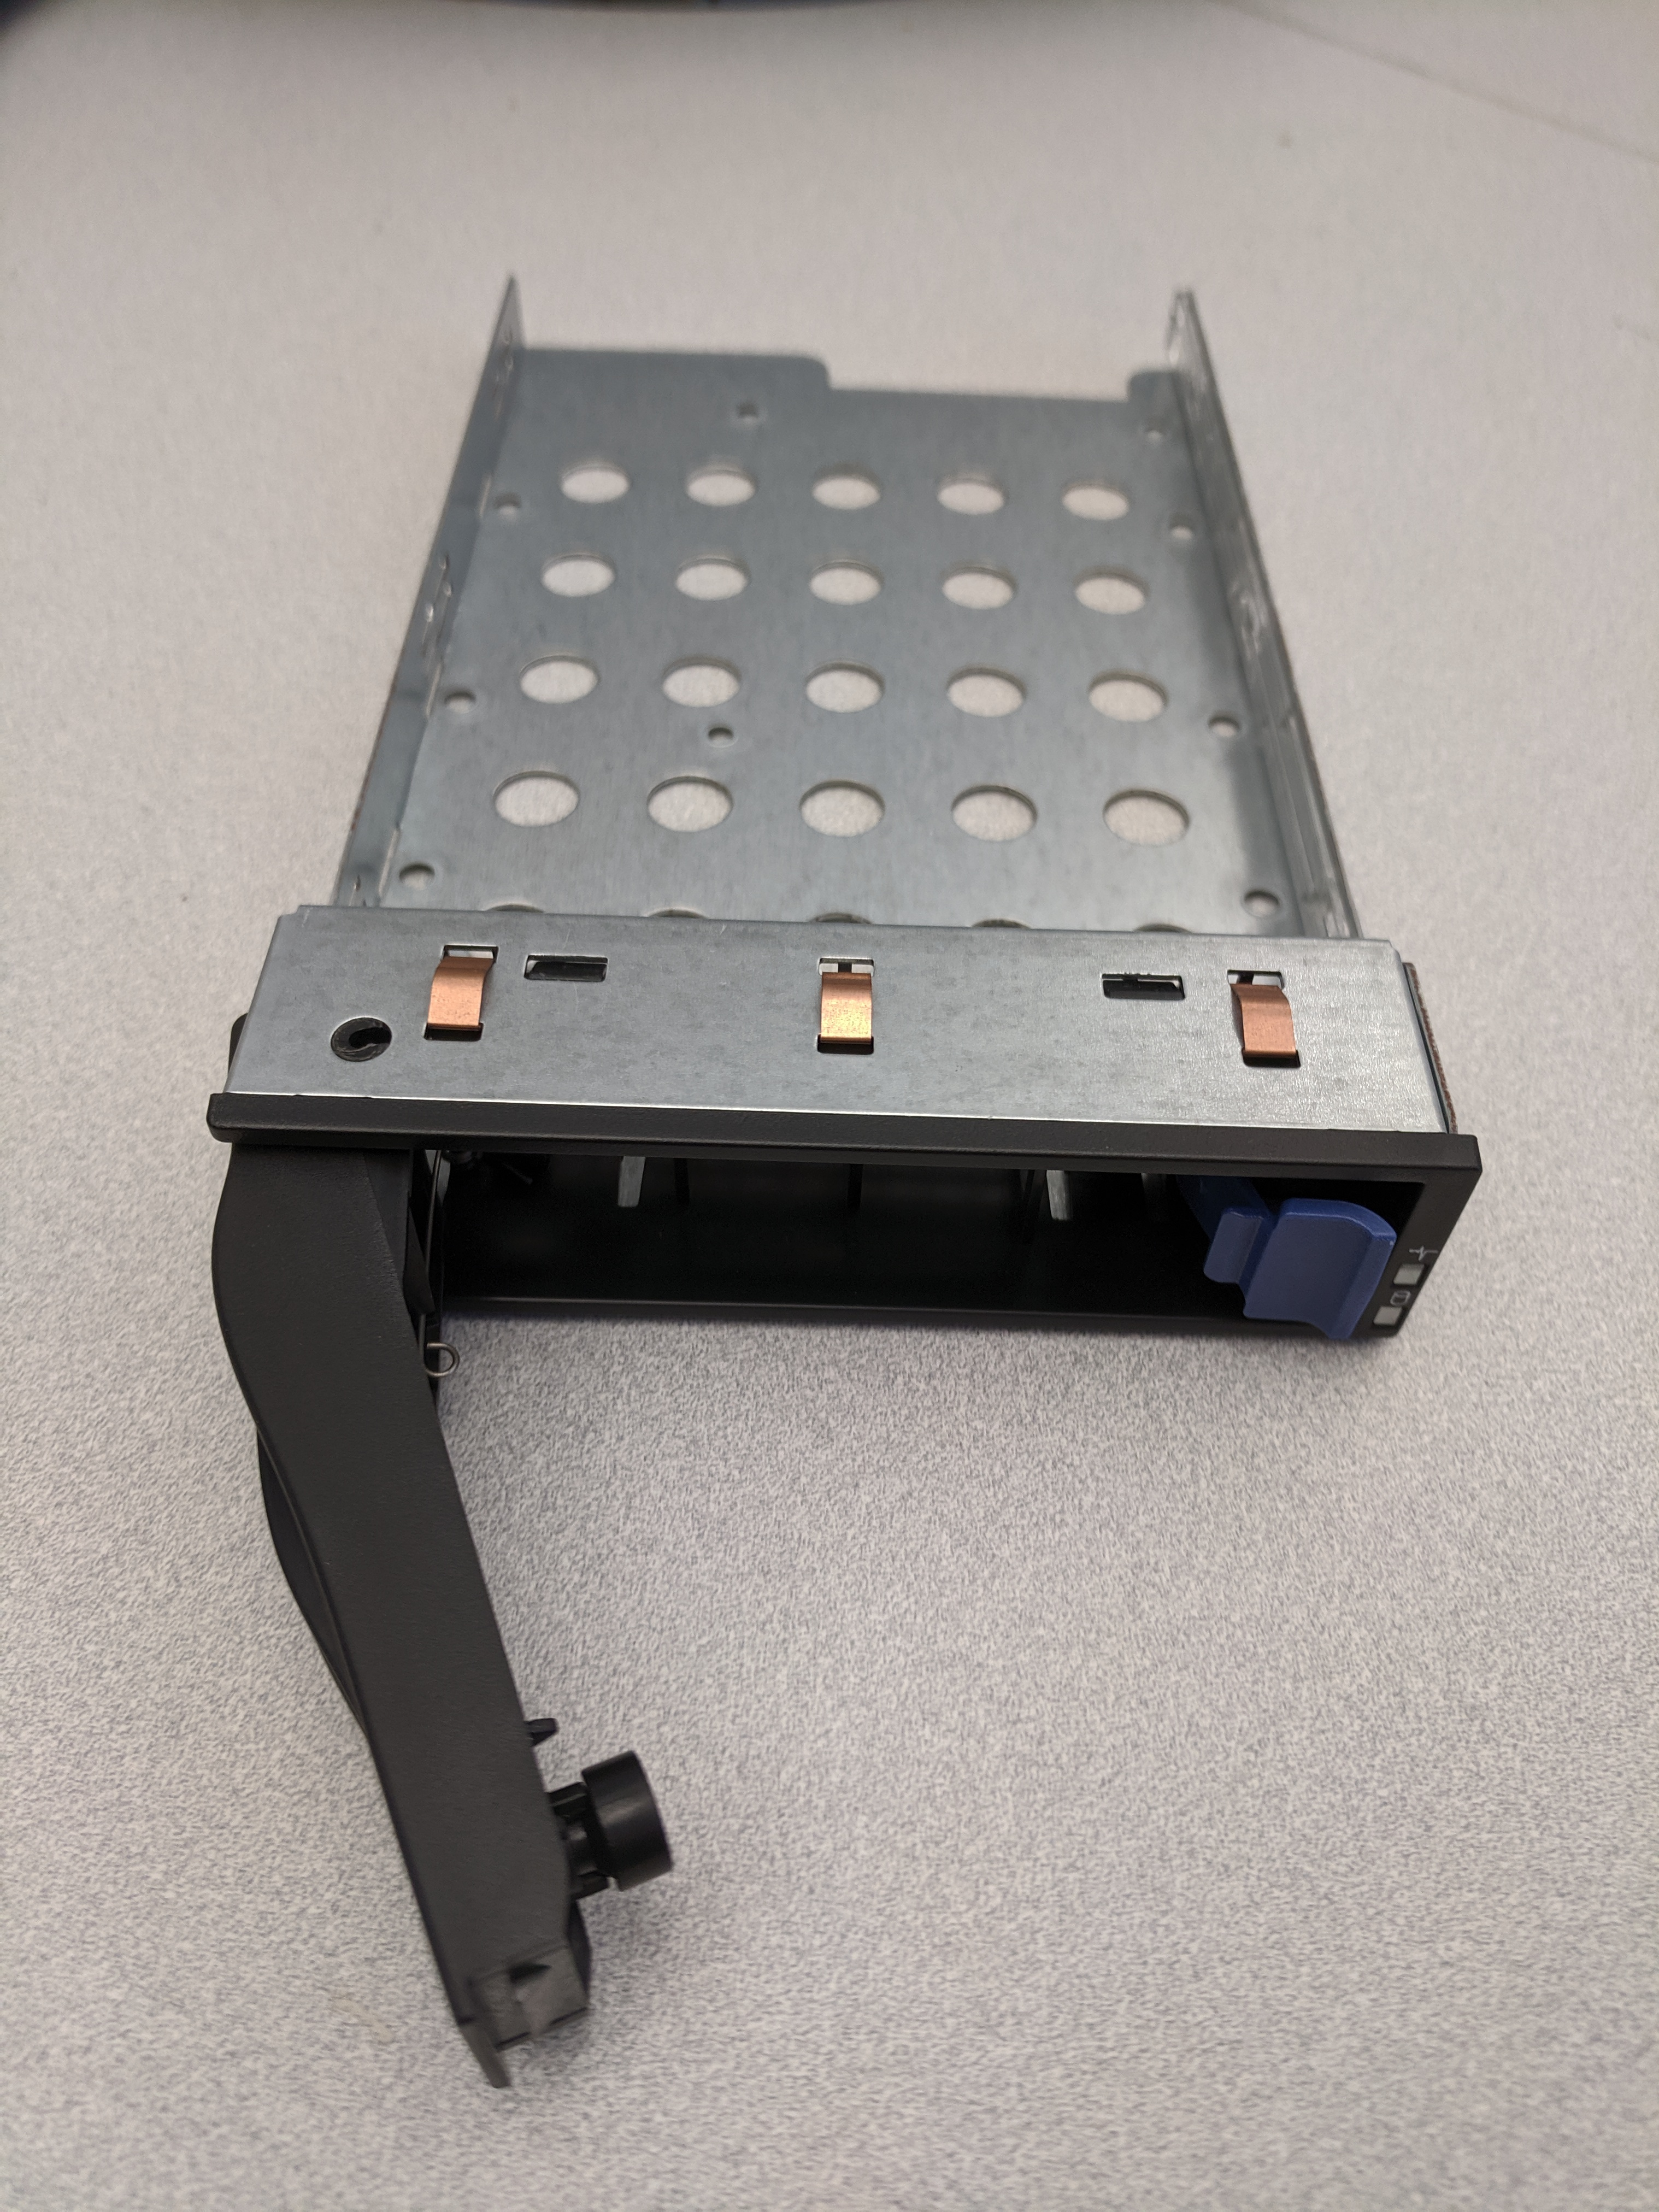
\includegraphics[width=0.3\linewidth]{FIGS/disktray.jpg}
\caption{Assembled DiskTray}
\label{fig:disktray}
\end{figure}

\begin{figure}
\centering
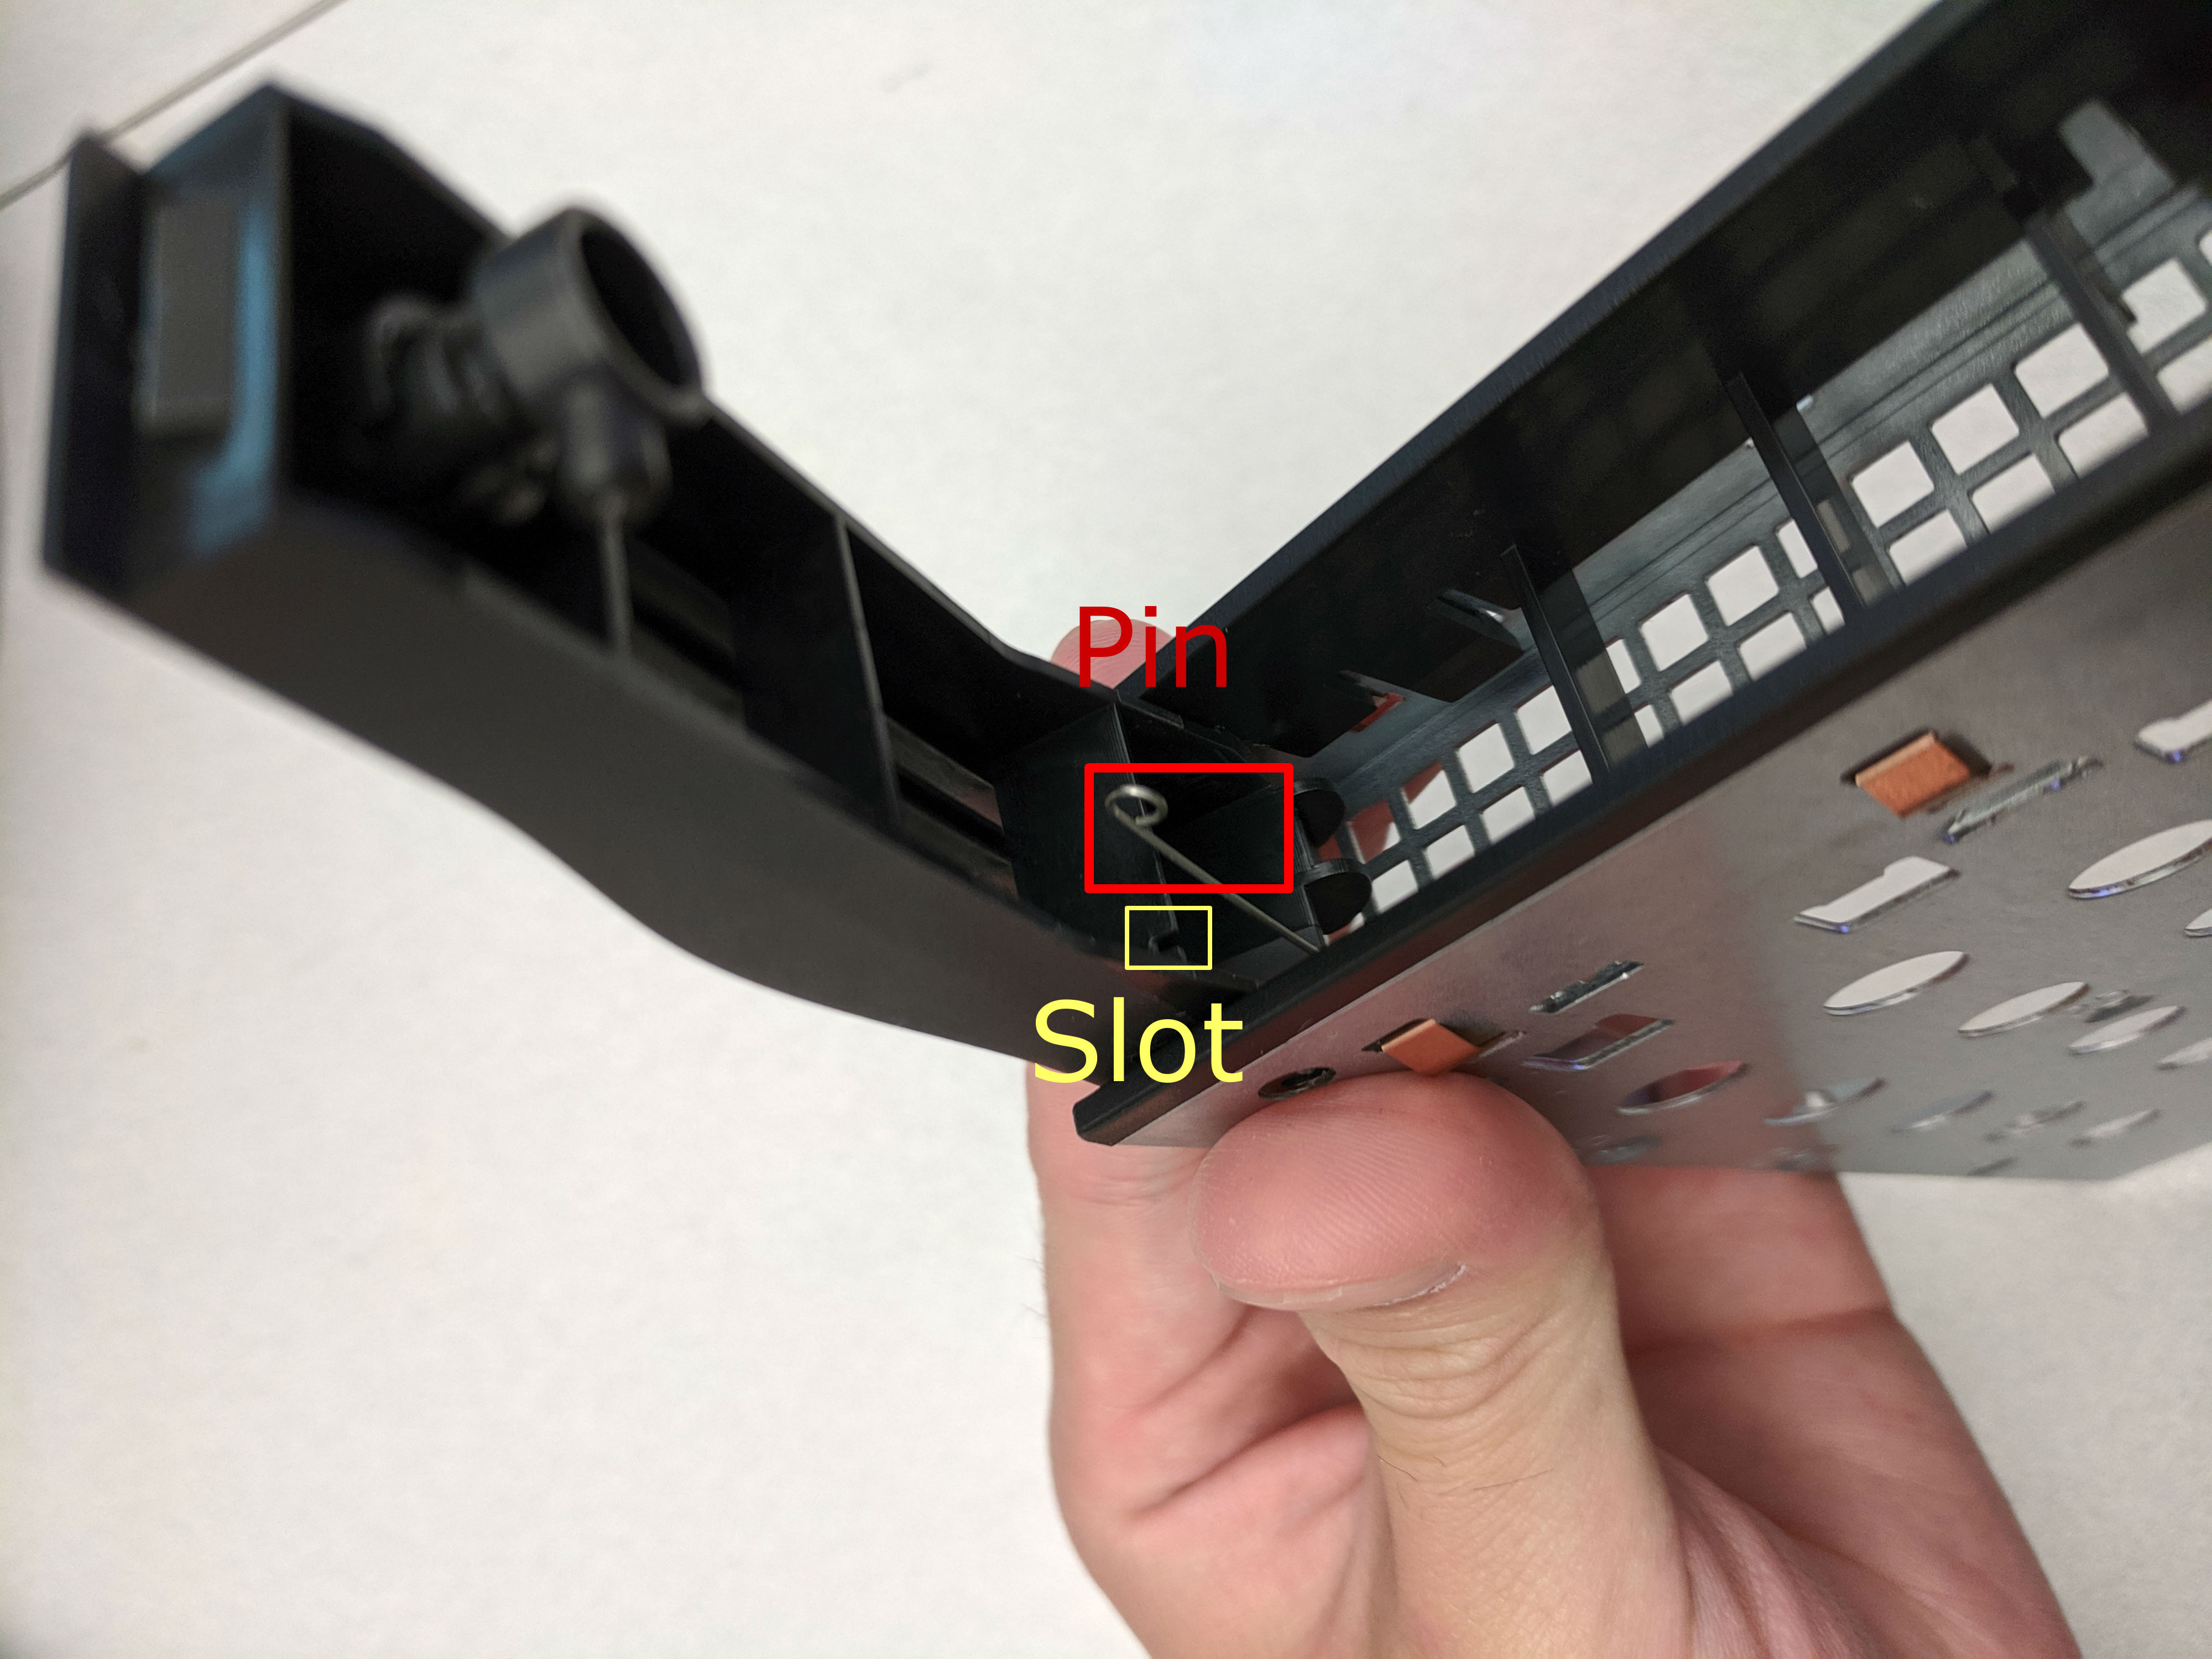
\includegraphics[width=0.5\linewidth]{FIGS/disktray-challenge.jpg}
\caption{Small Parts in DiskTray WCA}
\label{fig:disktray-challenge}
\end{figure}

In collaboration with InWin~\cite{inwin}, a computer hardware manufacturer, we
created a cognitive assistance to train operators how to assemble their disk
tray product. Figure~\ref{fig:disktray} shows the assembled tray, which is used
to host hard drives that go into a server chassis. As with all the other WCAs,
we do not modify the original parts. 

We face two challenges when building this application. First, some parts are
tiny. In one step, the application needs to check if a pin is placed correctly
into a slot. As shown in Figure~\ref{fig:disktray-challenge}, both the slot and
the pin are tiny and hard to see. To facilitate the detection of these two
parts, we ask the user to bring the parts close to the camera in addition to
zooming the camera and turning on the camera flashlight. Second, there is a
plastic strip that is translucent. Transparent objects are extremely challenging
to detect using 2D RGB cameras, because their appearance depends on the
background and lighting~\cite{lysenkov2013recognition}. Instead of detecting the
placement of the transparent strip by computer vision, we leverage the human
operator to signal to the system when the operation is completed. InWin
showcased this application at 2018 Computex Technology Show~\cite{computex}. A
demo video of the Computex Demo can be viewed
at~\url{https://www.youtube.com/watch?v=AwWZcL9XGI0}.


\section{Application Latency Bounds}

\begin{figure}
\centering
\begin{tabular}{|l|c|c|c|c|c|c|c|}
\hline
                      & POOL & WORK OUT & PING PONG & FACE &
                      \multicolumn{3}{c|}{
                          \begin{tabular}{@{}c@{}}Assembly Tasks\\ (e.g. RibLoc)\end{tabular}} \\
\hline
\Xhline{2\arrayrulewidth}
\hline
    Bound Range (tight-loose) & 95-105 & 300-500 & 150-230 & 370-1000 & \multicolumn{3}{c|}{600-2700} \\
\hline
\end{tabular}
\caption{Application Latency Bounds (in milliseconds)}
\begin{captiontext}
{\rm (Adapted from Chen et al~\cite{chen2017empirical})}
\end{captiontext}
\label{fig:bg-bounds}
\end{figure}

Not only are the accuracy of the instructions important to WCAs, but the speed
at which these instructions are delivered is also critical. With a human in the
loop, the latency requirements of WCAs are closely related to the task-specific
human speed. For example, for assembly tasks, an instruction delivered tens of
seconds after a user has finished a step can cause user annoyance and
frustration. For PING PONG assistant, a task that is even more fast-paced, an
instruction on where to hit the ball becomes useless if it is delivered after
the user has made a hit. 

Previous work~\cite{chen2017empirical} quantifies task-dependent application
latency bounds by answering the question \textit{How fast does an instruction
need to be delivered?} Three different approaches are used. For tasks that have
published human speed, numbers from the literature are used as the upper bound
of the end-to-end system response time. For example, it takes about 1000 ms for
a human to recognize the identity of a face. Therefore, a face recognition
assistant should deliver a person's name faster than 1000ms to exceed human
speed. For tasks in which users interact with physical systems, the latency
bounds can be derived directly from first principles of physics. For instance,
the latency bounds for PINGPONG assistant are calculated by subtracting audio
perception time, motion initiation time, and swinging time from the average time
between opponents hitting the ball. In addition, an user study of LEGO assembly
assistant is also conducted to deduct latency bounds for assembly tasks.

Figure~\ref{fig:bg-bounds} shows a summary of latency bounds calculated from the
previous work~\cite{chen2017empirical}. Each application is assigned both a
tight and a loose bound from the application perspective. The tight bound
represents an ideal target, below which the user is insensitive to improvements.
Above the loose bound, the user becomes aware of slowness, and user experience
and performance is significantly impacted. Latency improvements between the two
limits may be useful in reducing user fatigue.

These application latency bounds can be considered as application quality of
service (QoS) metrics. Similar to bitrate and startup time in video streaming,
these metrics serve as measurable proxies to user experience. When the system
delay increases, we can compare the delay with these latency bounds to estimate
how much a user is suffering. In this dissertation, we use these bounds to
formulate application utility functions, which quantify user experience when a
system response is delayed due to contention. These application utility
functions are the foundation for our adaptation-centered approach to
scalability.
